\subsection{Priprava okolja}
    Sam sem pri programiranju uporabljal operacijski sistem Ubuntu, popularno distribucijo Linuxa, ker je po mojem mnenju programiranje na Linuxu veliko lažje in bolj praktično kot na Windowsih. Tudi programski jezik Python je že prednaložen na večini Linux distribucijah, tako verzija 2.x kot 3.x. Program je napisan v Pythonu verzije 3.5.

    Najprej naložimo knjižnjici, ki jih potrebujemo:

    \inputminted[firstline=1, lastline=2, frame=lines]{bash}{latex/bashscripts.sh}


\subsection{Skrivanje podatkov}
    % vpisovanje gesla

\subsection{Iskanje podatkov}

\subsection{Primer uporabe programa}
    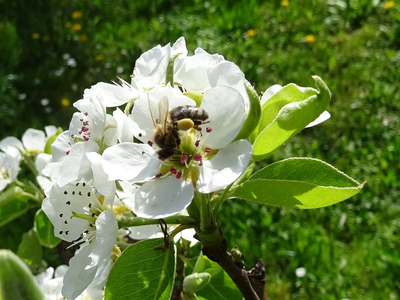
\includegraphics[width=0.5\textwidth]{image.png}
    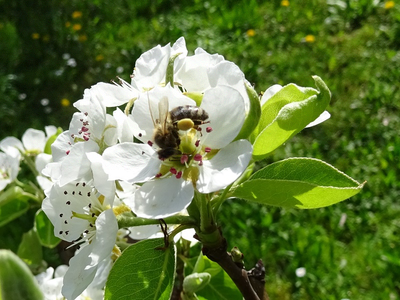
\includegraphics[width=0.5\textwidth]{image_with_hidden_data.png}

    Leva fotografija je samo fotografija čebele na cvetu, velika 400x300 slikovnih točk. Desna slika ji je na prvi pogled enaka, vendar je v njej skrito $10 000$ besed vzorčnega teksta (\textit{Lorem ipsum dolor sit amet\ldots}), zakriptiranih z geslom ``\texttt{geslo}''. Velikost datoteke, ki smo jo skrili je bila 68,1 kB. Prva slika je velika 254,5kB, druga pa 273,3 kB. Sliki se razlikujeta v velikosti, saj zaradi skritih podatkov v najnižjih bitih stiskanje podatkov ni bilo več tako zelo učinkovito. Razlika v velikosti v tem primeru ni bistvena, saj je prva slika že dovolj ``nepravilna'', da že prej ni bilo mogoče slike popolnoma stisniti. Če bi podatke skrivali v sliko, ki bi bila enobarvna, potem bi se velikost spremenila še bolj, poleg tega pa bi bilo s prostim očesom možno opaziti, da je v sliki nekaj skrito (slika ne bi bila več enbarvna, temveč bi bili sosednji piksli med seboj rahlo različnih barv).


    Program lahko uporabljamo na dva različna načina: v grafičnem načinu, ter v načinu ukazne vrstice.

    \subsubsection{Z ukazno vrstico}

        Recimo da imamo datoteko \texttt{slika.png}, v katero želimo skriti naše podatke, ki jih imamo spravljene v datoteki \texttt{skrivnost.txt}. Ime nove slike, v kateri bodo skriti podatki po \texttt{slika2.png}. Program iz ukazne vrstice pokličemo tako:

        \inputminted[firstline=4, lastline=5, frame=lines]{bash}{latex/bashscripts.sh}

        Program nas vpraša za geslo s katerim želimo kriptirati naše podatke, potem pa začne s skrivanjem podatkov v sliko. Ker je slika lahko velika in lahko skrivanje traja nekaj 10 sekund, program sproti prikazuje kako daleč je prišel.

        Če potem želimo najti podatke v sliki z imenom \texttt{slika.png} in jih shraniti v datoteko \texttt{nova\_skrivnost.txt}

        \inputminted[firstline=7, lastline=7, frame=lines]{bash}{latex/bashscripts.sh}

    \subsubsection{Z grafičnim vmesnikom}
        Prav tako je vse mogoče narediti s preprostim grafičnim vmesnikom. Da ga zaženemo, v mapi \texttt{src/} izvedemo naslednji ukaz:

        \inputminted[firstline=9, lastline=9, frame=lines]{bash}{latex/bashscripts.sh}

        Izberemo sliko, v katero želimo skriti podatke, vpišemo geslo za kriptiranje, ime nove slike in datoteko, ki jo želimo skriti. Prav tako lahko s pomočjo grafičnega vmesnika pridobivamo skrite podatke iz slik.

        \centering
        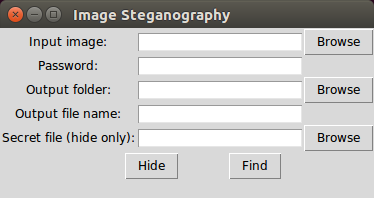
\includegraphics[width=0.6\textwidth]{program_screenshot.png}
